\documentclass[12pt,english]{article}
\usepackage{geometry}
\usepackage{float}
\usepackage{caption}
\geometry{verbose,tmargin=3cm,bmargin=3cm,lmargin=3cm,rmargin=3cm}
\usepackage{amsmath}
\usepackage{amssymb}
\usepackage{amsthm}
\usepackage{verbatim}
\usepackage{adjustbox}
\usepackage{hyperref}
\usepackage{graphicx}
\usepackage{setspace}
\usepackage{changepage}
\onehalfspacing
\usepackage{babel}
\newcommand{\expec}{\ensuremath{\mathbb E}}
\begin{document}
\begin{center}
{\Large{}Section 8: Education quality and cost effectiveness} \\
{\large{}Duflo, Hanna, and Ryan (2012), Kremer, Brannen, and Glennerster (2013)}
\par\end{center}{\Large \par}

\begin{center}
EEP 152
\par\end{center}

\begin{center}
October 26, 2016
\par\end{center}

\begin{itemize}
	\setlength\itemsep{-0.5em}
	\item CEA (30 min)
	\item DHR (10 min)
	\item CEA (DHR,  KBG) (10 min)
\end{itemize}
A copy of a public version of the papers, along with the section notes, are available on the section Github at \href{github.com/johnloeser/eep152}{github.com/johnloeser/eep152} in the ``section8'' folder.

\section{CEA}

\subsection{Definition}

Last week, we discussed the consistent finding that investment in education has positive social benefits. Using a cross-country regression and two natural experiments involving primary school construction, we found that increasing attendance by 1 year/student increases average earnings by 8\%-15\%. Does this mean we should build primary schools?

Maybe -- it depends on the costs of the construction, and the associated increase in earnings.\footnote{Plus any other benefits of increases in education. For example, it's possible that increased education causes increased civic engagement.} We can calculate this formally in a cost-benefit analysis framework (CBA), using a fixed discount rate, to compare the costs and benefits of school construction.\footnote{Duflo performs exactly this analysis in her 2001 paper; you can read Section VI of that paper if you're curious about the methodology. She finds that the program appeared to have had significant, economically and statistically, positive net benefits.}

$$ \text{Benefits} = \sum_{t = 1973}^{\text{future}} \underbrace{\delta^{t - 1973}}_{\text{discount factor}} \times \text{Benefits}_{t} $$

$$ \text{Costs} = \sum_{t = 1973}^{\text{future}} \underbrace{\delta^{t - 1973}}_{\text{discount factor}} \times \text{Costs}_{t} $$

$$ \text{Net benefits} = \text{Benefits} - \text{Costs} $$

We can sum the costs and benefits of the program over each period in which the program had costs (the years during which schools were being built) and benefits (the years during which the extra students who attended school were receiving higher earnings), discounting later periods relative to earlier periods. After computing this sum, we'd consider primary school construction a ``good program'' if the net benefits are positive.

However, it is often the case that governments are constrained. It's possible, for example, that the government of Indonesia had a finite education budget in 1973, and as a result it could not spend money on every single program with a positive net benefit. Given this constraint, how should the government decide which programs to invest in?

An alternative metric to CBA is to use cost effectiveness analysis (CEA). Instead, we can calculate
$$ \text{Cost Effectiveness} = \frac{\text{Benefits}}{\text{Costs}} $$
which is the benefit per unit of expenditures. This is the metric that would be most relevant to the policy maker in our hypothetical case -- they would like to know which programs generate the most benefit per unit of expenditure, so they could undertake the most cost effective programs first. This is a common concept in economics -- for example, many economists support a carbon tax because it means that any unit of emissions with a cost of abatement less than the carbon tax will be stopped, while any unit of emissions with a cost of abatement greater than the carbon tax will continue.\footnote{The McKinsey curve is an example of the application of this reasoning for a carbon tax, although they report their numbers as $\frac{\text{Costs}}{\text{Benefits}}$.} Similarly, a policy maker following this rule will not make any investment that could be substituted for other investments which would generate greater benefits with the same expenditure.

If this seems abstract, this exact exercise was performed recently by a think tank for the government of Bangladesh across a broad menu of programs, and is described in an \href{http://www.economist.com/news/finance-and-economics/21698302-ambitious-attempt-work-out-best-use-scarce-resources-how-spend-it}{Economist article} titled ``How to spend it''. However, as mentioned in the article, attempting to do this across all categories of expenditures is extremely ambitious -- different estimates of cost effectiveness may vary dramatically in quality, and comparing the cost effectiveness of military and education expenditures requires many assumptions.

\subsection{Application: School quality}

Going back to the example of the policy maker, suppose that our hypothetical policy maker is tasked with improving primary school quality with a fixed budget. They have a menu of programs at their disposal they could implement -- monitoring and incentives for teachers, uniforms or textbooks for students, scholarships, funding learning centers, changing the language of instruction, and others.

Suppose the policy maker wants to use CEA to decide which programs to pursue. The policy maker knows the costs of each program, and their annual budget. How can they calculate the benefits?

Ideally, we would have some measure of the effect of each program on welfare. Another advantage to CEA is that, by measuring a ratio instead of a difference, we no longer need costs and benefits to have the same units. While it will almost always make sense for costs to be in units of \$, we can think of alternative units for benefits -- QALYs in medicine, infections averted in public health, or even measures of inequality. Unfortunately, quantifying welfare is hard.

However, income is much easier to measure, and it's been observed that income, fairly robustly, predicts higher reported life satisfaction. Maximizing income also has the advantage that we're back in the same units, and we can compare expenditures on education to reducing taxes (which will increase income by about \$1 per \$1 of expenditures). However, it may be the case that the policy maker is operating in a country that won't redistribute the gains from the program -- as a result, a program that increases rich students' incomes might be valued less than a program that increases poor students' incomes. We can use a concave function of income (such as square root of income, or more commonly log of income) to capture this. However, not every impact evaluation has the ability to collect data on long run effects, as Duflo (2001) was able to for school construction. If we don't know the effects of monitoring and incentives for teachers or free uniforms for students on long run incomes, how should we choose between the two programs?

An alternative is to use a proxy or surrogate for income -- something that strongly predicts future income. Test scores are one plausible candidate. For example, in the United States, Chetty, Friedman, and Rockoff (2014) find that a 1 standard deviation (sd) increase in test scores is associated with a 1.3\% increase in earnings. If test scores allow us to measure the learning that eventually makes students more productive, then we can use test scores to capture the benefits of these interventions.

Kremer, Brannen, and Glennerster (2013) (KBG) perform exactly this exercise, and produce the following figure.
\begin{figure}[H]
\caption{Education quality CEA from KBG}
\centering
\resizebox{\textwidth}{!}{
	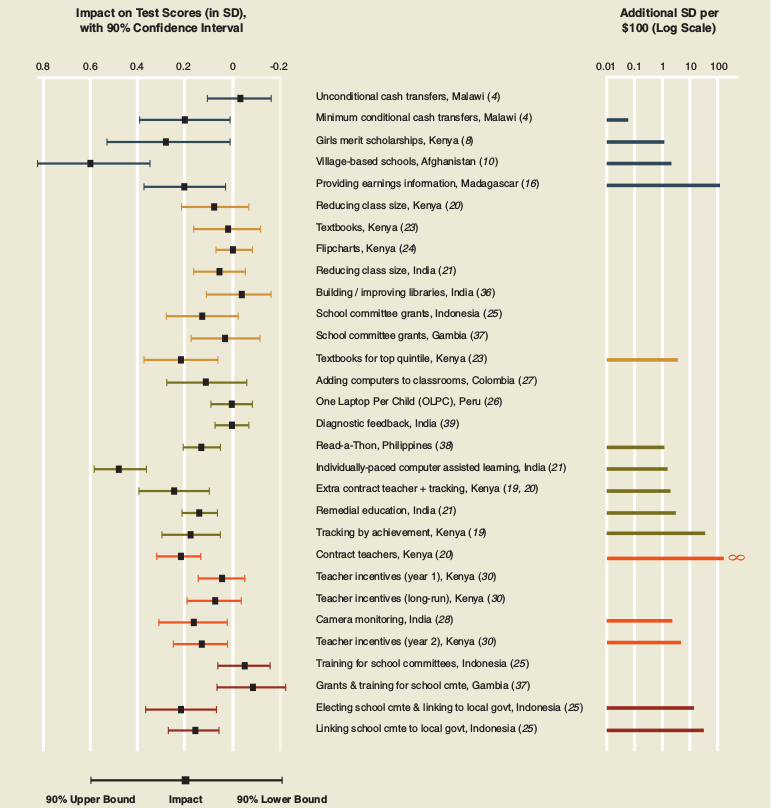
\includegraphics{fig1}
}
\end{figure}
How should we interpret this figure? Some extremely cost effective programs (such as changes in school governance structures) may have limited external validity, since the effect of the program may vary with characteristics of the context within which it's implemented. Additionally, some large estimated effects may actually be very small, due to wide bounds on the confidence interval on effects on test scores. As we discussed during microfinance, conducting a meta-analysis across multiple studies in different contexts can help to resolve these problems after a body of evidence has been developed.

More difficult to resolve is that some of these interventions may produce "lower quality" increases in test score sd than others. This is possible for a number of reasons.

First, given an intervention that targets test scores and an intervention that does not, both of which result in the same increase in test score sd per \$100 of expenditures, the intervention that does not target test scores is likely to have larger long term impacts. To see this, consider the case of paying teachers based on test scores and paying teachers based on qualitative evaluations of soft skills. If both increase test score sd the same amount, then it's likely that students whose teachers were paid based on qualitative evaluations of soft skills learned more than other students. To give another example of this, health interventions which also affect school attendance or test scores are likely to have much larger positive effects on long term outcomes than educational interventions which more directly target school attendance or test scores and have the same short term effects.

Second, some of these interventions may be easier to scale up than others. Actual attempts to supply textbooks might have high leakage due to corruption, while incentives may have different short run and long run effects. As an alternative case, although the camera intervention seems difficult to scale, the implementing partner for that project, \textit{Seva Mandir}, cheaply scaled that intervention across all their NFEs after the success of the RCT. Other RCTs above, such as cash transfers, may have already been evaluated at scale.

Finally, measuring test scores in standard deviations allows comparison across contexts, but that does not necessarily mean the same increase in test scores across two contexts is equivalent. Different tests measure different skills, and different tests measure those skills with different precision.

\subsection{DHR}

As we discussed in class, DHR provide cameras (used for monitoring attendance) and incentives to attend to a random 60 out of 120 schools in partnership with \textit{Seva Mandir}, an NGO in India which runs nonformal education centers (NFEs).

DHR can evaluate the program with a simple difference -- they can compare outcomes on a mid-test and a post-test for students attending treatment schools (where the teachers received a camera and incentives to attend) to control schools (where nothing changed). In doing so, they find an approximately 0.2 sd increase in test scores in the treatment group relative to the control group.

Why did \textit{Seva Mandir} decide to scale up the program? Since attendance was incentivized, in addition to measuring test scores, DHR monitor attendance and teaching performance using \textit{Seva Mandir}'s standard randomized audits. They find that teachers do not change how they're teaching, but they do attend more, and that the attendance effect persists over time.

\begin{figure}[H]
	\caption{DHR: Effects on attendance}
	\centering
	\resizebox{\textwidth}{!}{
		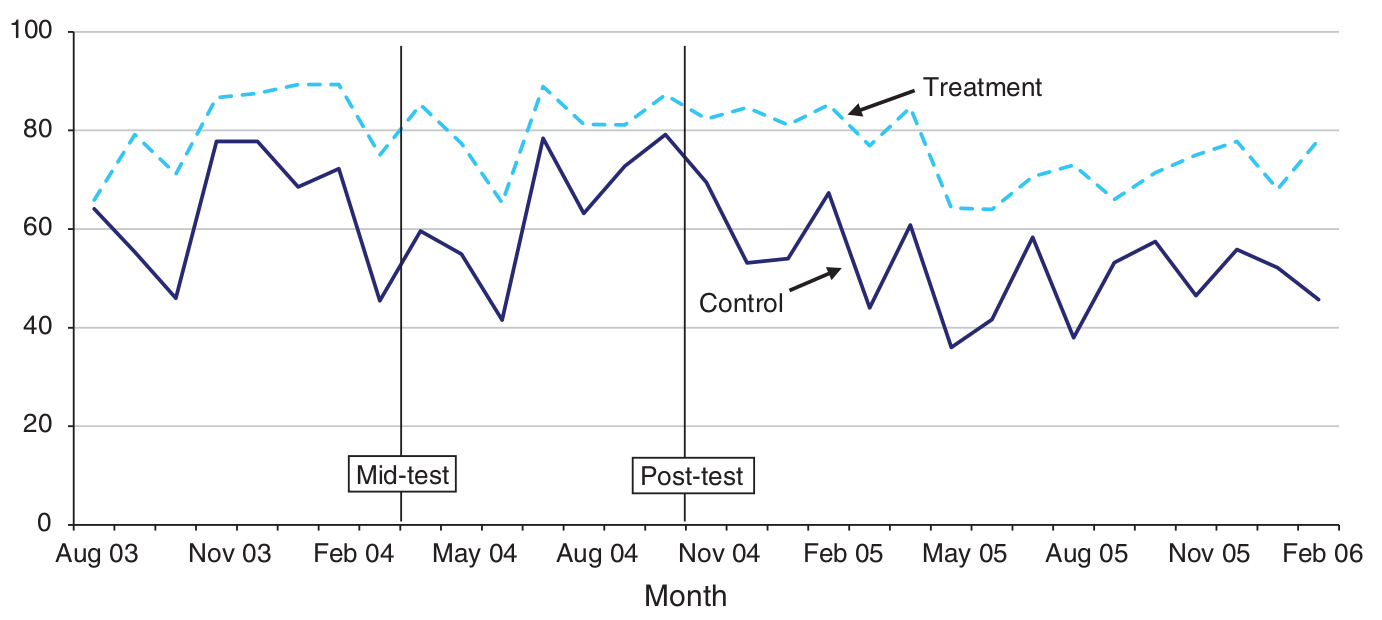
\includegraphics{fig2}
	}
\end{figure}

Additionally, although this isn't relevant to calculating the overall cost effectiveness of monitoring and incentives combined, DHR also argue that the effect on attendance is significantly driven by incentives. To see this, they rely on the fact that teachers attendance was only incentivized if those teachers attended 10 or more days in a given month. We can imagine a DID framework then -- teachers who attended less than 10 days before the last day of a given month can be compared to teachers who attended at least 10 days before the last day of a given month, and they can be compared on their behavior on the last day of the month relative to their behavior on the first day of the next month.

\begin{figure}[H]
	\caption{DHR: Effects of incentives}
	\centering
	\resizebox{\textwidth}{!}{
		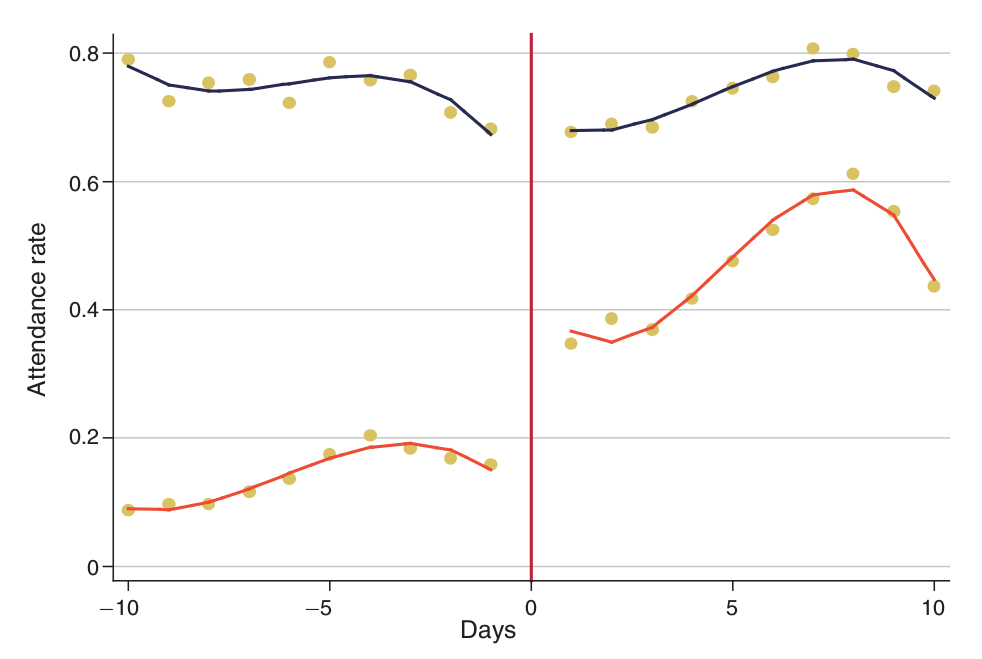
\includegraphics{fig3}
	}
\end{figure}

The top line is teachers who attended 10 or more days in a given month -- their attendance does not change moving from the last days of that month to the first days of the next month, since their incentives to attend are roughly the same in both months. The bottom line is teachers who attended less than 10 days in a given month -- their attendance increases significantly from the last day of that month to the first day of the next month, when they again have an incentive to attend.

\subsection{Application: DHR}

How should we calculate the cost effectiveness of DHR? Fortunately, we don't have to on our own -- you can see KBG perform the calculation, and we can go to \href{https://www.povertyactionlab.org/policy-lessons/cost-effectiveness}{J-PAL's website} to get an email address for someone who has information on the exact calculation, and where the $\approx 2\;\text{sd}/\$100$ ratio comes from.

We can try to back out the costs that they used. First, since the program is being scaled, lets assume the fixed costs are minimal (which includes administrative expenses in delivering incentive payments and analyzing the attendance data from the cameras). The cost of the program is the initial cost of the camera, paid in the first year, plus the additional incentive payments made to teachers. The benefits of the program is the annual 0.2 sd increase in test scores per student. Lets further assume that the expected lifetime of a camera is 5 years, and that the discount rate used in India is 12\%.\footnote{This is lifted from Dhaliwal, Duflo, Glennerster, and Tulloch (2013). In the case of India, this number was calculated as the social opportunity cost of capital, which is the assumed amount of costs society would incur if the government deferred its least cost effective expenditures by one year.} Let $x$ be the cost of the camera. Additionally, since the targeted attendance (20 days per month) was the same in treatment and control, lets assume that the average incentive payment was 0. This yields
$$ \text{Benefit} = \sum_{t = 0}^{4} \underbrace{(1 - .12)^{t} }_{\text{discount factor}} \times \; 20 \; \text{students} \times 0.2 \; \frac{\text{sd}}{\text{student}} \approx 16 \text{sd} $$
$$ \text{Cost} = \sum_{t = 0}^{0} \underbrace{(1 - .12)^{t} }_{\text{discount factor}} \times \$ x = \$ x $$
$$ \text{Cost effectiveness} = \frac{\text{Benefit}}{\text{Cost}} \approx 2 \; \frac{\text{sd}}{\$100} \Rightarrow x \approx \$ 800 $$
Clearly, there are some other costs we're missing that KBG use in their calculation. The administrative costs we assumed away might be significant. Setting administrative costs to be \$150/year,\footnote{If one monitor can monitor attendance of 10 teachers, this implies a cost per monitor of \$1500, which is plausible.} and the cost of a camera to be \$200\footnote{This is 2003, pre-Shenzhen boom, that we're talking about.}, we get
$$ \text{Cost} = \$ 200 + \left( \sum_{t = 0}^{4} \underbrace{(1 - .12)^{t} }_{\text{discount factor}} \times \$ 150 \right) \approx \$ 800 $$
$$ \text{Cost effectiveness} \approx 2 \; \frac{\text{sd}}{\$100} $$
which is the same number as KBG.


\end{document}